\documentclass{article}
\usepackage{tikz}
\usetikzlibrary{external}
\usetikzlibrary{arrows}
%\tikzexternalize % activate!

\begin{document}
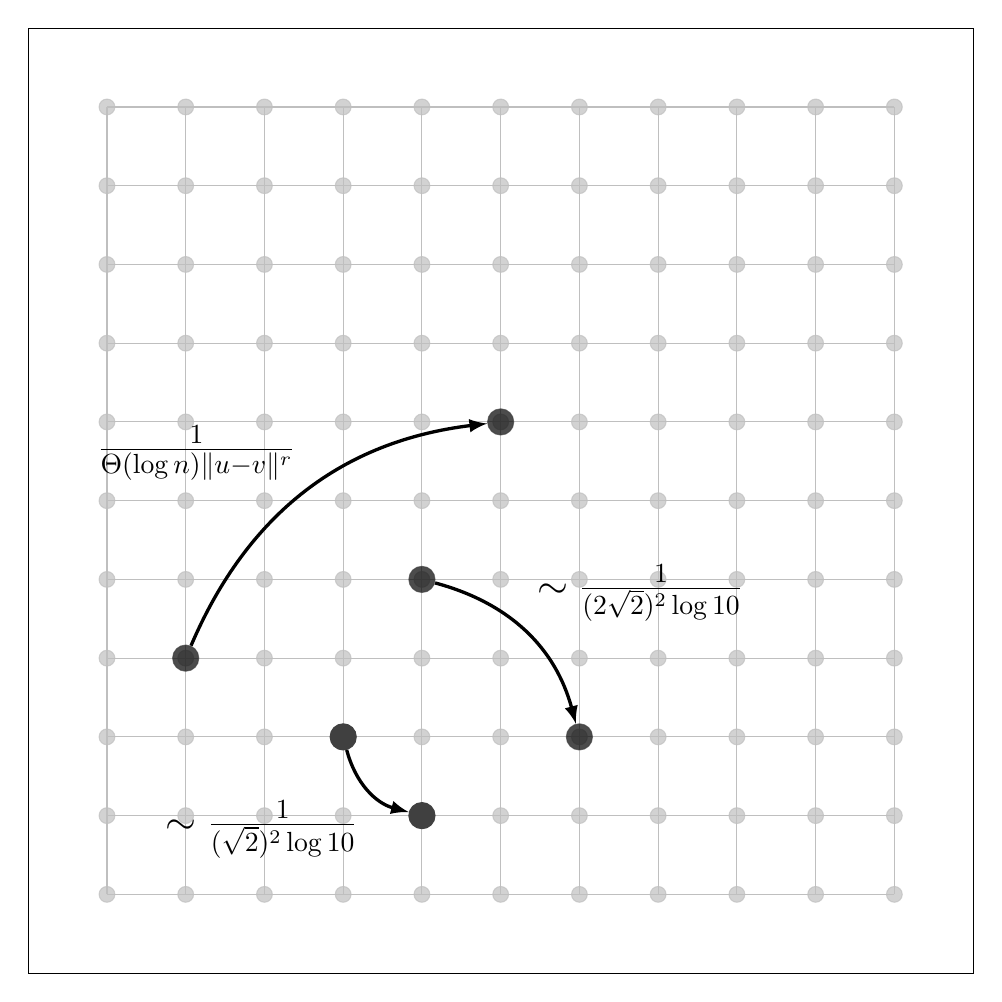
\begin{tikzpicture}[]
  \tikzset{style={font=\Large}}
    % Grid
    \draw[clip] (-1,-1) rectangle (11,11);
    \draw[step=1,color=lightgray] (0,0) grid (10,10);
    \foreach \xpos in {0, 1, 2, 3, 4, 5, 6, 7, 8, 9, 10}
    {
      \foreach \ypos in {0, 1, 2, 3, 4, 5, 6, 7, 8, 9, 10}
      {
      \draw [color=lightgray,fill=lightgray,opacity=0.7] (\xpos,\ypos) circle (0.1);
      };
    };

    % Some long paths

    \node (v1) [circle,draw,color=darkgray,fill=black,opacity=0.7] at (1,3) {};
    \node (v2) [circle,draw,color=darkgray,fill=black,opacity=0.7] at (5,6) {};
    \draw [overlay,-latex,very thick] (v1) to [bend left] node[above left, color=black, opacity=1.0] {$\frac{1}{\Theta(\log n) \|u-v\|^{r} }$} (v2);

    \node (v3) [circle,draw,color=darkgray,fill=black,opacity=0.7] at (4,4) {};
    \node (v4) [circle,draw,color=darkgray,fill=black,opacity=0.7] at (6,2) {};
    \draw [overlay,-latex,very thick] (v3) to [bend left] node[above right, color=black, opacity=1.0] {$\sim \frac{1}{(2\sqrt{2})^{2} \log 10}$} (v4);
    
    \node (v5) [circle,draw,color=darkgray,fill=darkgray] at (3,2) {};
    \node (v6) [circle,draw,color=darkgray,fill=darkgray] at (4,1) {};
    \draw [overlay,-latex,very thick] (v5) to [bend right] node[below left, color=black, opacity=1.0] {$\sim \frac{1}{(\sqrt{2})^{2} \log 10}$} (v6);

\end{tikzpicture}
\end{document}
